\chapter{Tool}

\section{Obiettivi}

Il progetto che si è scelto di realizzare nell'ambito della tesi consiste in uno strumento per effettuare acceptance test di applicazioni web. E' importante chiarire gli obiettivi che si sono prefissati per comprendere meglio alcune delle scelte che sono state fatte circa le funzionalità e l'architettura del software realizzato. Esso si differenzia dalle soluzioni open source presentate in precedenza principalmente per la tipologia di test per il quale è pensato e per le competenze che sono richieste nell' utilizzo.

Come si è visto, esistono svariati sistemi molto validi per effettuare test su di una applicazione web. Essi sono stati sviluppati principalmente per offrire agli sviluppatori uno strumento in grado di automatizzare l'esecuzione di test sull'interfaccia grafica e di facilitare la scrittura di test per diversi browser. Analogamente a quanto avviene per altre metodologie, affinché l'insieme dei test scritti per l'interfaccia sia efficace e possa seguire la naturale evoluzione dell'applicazione senza richiedere alti costi di mantenimento, è necessario poter sfruttare competenze nell'ambito dell'ingegneria del software, strettamente legate a quelle richieste per lo sviluppo dell'applicazione stessa. 

In altri termini, un'attività di testing produttiva, completa ed efficace non può essere improvvisata, ma deve essere condotta da programmatori con esperienza in questo ambito. Come diretta conseguenza, la maniera più rapida e flessibile per automatizzare i test sulle interfacce grafiche consiste nello scrivere le verifiche in maniera programmatica utilizzando un framework, come ad esempio Watir, che solleva dallo sviluppatore il peso di dover adattare i test per i vari browser e che semplifica notevolmente alcune operazioni di frequente utilizzo.

Sebbene infatti si siano analizzati diversi strumenti per registrare automaticamente le operazioni da eseguire durante i test, essi non possono fornire la potenza e la flessibilità di un test scritto in maniera programmatica, che può sfruttare l'espressività di un linguaggio di programmazione. Gli stessi sviluppatori di Selenium IDE ne propongono l'utilizzo per velocizzare la scrittura dei test, grazie alle funzioni di esportazione, utilizzando i comandi messi a disposizione dall'API Selenium WebDriver, presentandolo come un tool complementare e non autosufficiente per l'esecuzione di test approfonditi ed efficaci. 

Dopo l'utilizzo pratico di alcune delle soluzioni presentate, è emerso infatti che gli strumenti di registrazione ed esecuzione automatica, a causa della loro intrinseca natura visuale, non permettono ad esempio di adattare in maniera rapida il test acquisito rispetto a modifiche effettuate sull'interfaccia grafica. Nella maggior parte dei casi sarebbe quindi necessario registrare nuovamente il test, operazione che può essere anche molto onerosa in termini di tempo a seconda del numero di test interessati. Nelle stesse condizioni, l'impiego di test scritti in maniera programmatica consente al contrario di riutilizzare frammenti di codice già esistente per ridurre notevolmente le modifiche necessarie ad adeguare il test ai cambiamenti nella struttura dell'interfaccia. A questo proposito Selenium WebDriver propone un pattern di scrittura dei test chiamato Page Objects pattern (\cite{pageObject}), che suggerisce di aggiungere un livello di indirezione tra il codice dei test e l'interfaccia, per incapsulare in oggetti l'associazione tra gli elementi dell'interfaccia grafica e le funzionalità da essa esposte.

Queste considerazioni sono generalmente valide per i test di integrazione e i test funzionali, che sono scritti e mantenuti da un team di programmatori e hanno l'obiettivo di verificare il corretto funzionamento dell'interfaccia grafica dell'applicazione web. Bisogna però tenere in considerazione che l'integration testing ed il functional testing hanno degli scopi ben delineati e che ottengono risultati positivi solo se vengono applicati nei loro domini di competenza e in fasi precise all'interno del ciclo di sviluppo del software. 

L'acceptance testing, come si è evidenziato all'inizio della trattazione, viene effettuato per assicurarsi che lo sviluppo del software segua i requisiti indicati dal committente. Così come è importante stabilire con chiarezza i requisiti dettati dalle business rules e verificarli costantemente durante il ciclo di sviluppo, è allo stesso modo opportuno seguire una strategia analoga per quanto riguarda i requisiti posti sull'interfaccia grafica dell'applicazione.  
Chi si occupa dello sviluppo potrebbe essere portato dal suo ruolo a sottovalutare l'importanza che riveste l'interfaccia grafica nella visione dell'utente finale. Se quest'ultima non rispecchia le esigenze reali di utilizzo, poiché ad esempio non presenta i dati in maniera efficace o rende macchinose operazioni utilizzate di frequente, di fatto diminuisce notevolmente il valore percepito dal committente e può vanificare facilmente tutti gli sforzi compiuti ai livelli meno visibili dell'architettura dell'applicazione. 

A riprova di ciò, si può notare che spesso il committente esprime i propri requisiti sul software proprio partendo dall'interfaccia grafica. Questo avviene naturalmente poiché essa è per definizione il punto di contatto tra la persona che utilizza l'applicazione e le funzionalità che essa espone. E' sicuramente compito degli sviluppatori collaborare con il committente per tradurre questi requisiti in business rule generiche, che esulano dall'implementazione grafica, ma sarebbe comunque una perdita notevole di informazione non formalizzare in aggiunta anche i dettagli d'uso espressi sull'interfaccia.

Partendo da questi presupposti, lo strumento che si andrà a sviluppare dovrà poter essere utilizzato anche da persone senza competenze tecniche particolari, in modo che i test di accettazione possano essere definiti ed eseguiti anche da figure professionali che appartengono all'organizzazione del committente, in autonomia o in collaborazione con gli sviluppatori. L'impiego previsto pone dunque diversi vincoli sulle scelte implementative e sugli obiettivi funzionali di tale strumento, che verranno ora descritti più in dettaglio.

\subsection{Facilità di utilizzo}

Come appena scritto, non vengono richieste competenze tecniche per l'utilizzo dello strumento. Se l'utente le possiede, potrà decidere di impiegarle per accedere ad alcune funzionalità avanzate. In caso contrario comunque la definizione, l'esecuzione e l'analisi del risultato degli acceptance test sull'interfaccia grafica dell'applicazione web dovranno essere comunque di facile e veloce realizzazione. 

Questo requisito esclude in grande misura la possibilità di utilizzare gli strumenti analizzati nei capitoli precedenti. Le librerie per l'automazione dei browser richiedono notevoli competenze nell'ambito della programmazione, quindi il loro impiego da parte del committente o comunque di persone esperte del dominio del business è da escludersi, rispetto agli scopi prefissati. Si ricorda che ciò non implica l'inutilità di questi sistemi: semplicemente il loro target d'uso e il livello di astrazione interessati dai test sono differenti rispetto a quelli richiesti nell'analisi fatta finora. 

Sono inoltre poco adatti allo scopo anche gli strumenti di registrazione automatica, come Selenium IDE o Windmill visti in precedenza. Sebbene essi rendano la fase di definizione e di verifica più accessibile poiché non richiedono competenze di programmazione, in realtà sottintendono la conoscenza di alcune tecnologie utilizzate nello sviluppo dell'applicazione, quali CSS, HTML, e XPath. 
Per effettuare un confronto, si prenda in esame l'estensione Selenium IDE. Essa ad esempio non consente all'utente di specificare il nodo del DOM interessato da una assertion in maniera visuale, ma richiede di inserirne manualmente un selettore XPath o CSS; è possibile facilitare questo compito usando estensioni addizionali come Firebug, che richiedono comunque una certa familiarità con il concetto di selettore e di DOM. 

Anche con le giuste competenze, l'identificazione di questo selettore non è di fatto assistita in alcun modo. Questo fatto costringe all'impiego di altri strumenti aggiuntivi e che spesso porta  percorsi XPath più complessi del necessario e decisamente poco flessibili per quanto riguarda le modifiche successive che potranno interessare l'interfaccia. Poiché non viene proposta una strategia assistita, aumenta la probabilità di commettere errori e cresce notevolmente la quantità di tempo necessaria per definire i test, con un conseguente aumento di costi tale da scoraggiare l'automazione dei test di accettazione. 

Inoltre, per specificare che tipo di verifica si intenda fare, è necessario in SeleniumIDE selezionare il comando più adatto tra l'elenco di funzioni messe a disposizione da WebDriver. Anche in questo caso è richiesta una certa competenza nell'utilizzo di questa libreria, che è molto potente ma prevede oltre un centinaio di comandi solamente per definire la tipologia di assertion che si intende effettuare.

Sempre dal punto di vista della facilità d'impiego e delle competenze richieste, Windmill risulta più complicato di Selenium IDE, sia perché l'interfaccia grafica risulta poco organizzata e accessibile, sia perché anche in questo strumento non esiste un modo semplice per specificare il tipo di verifica che si intende eseguire. Esiste invece uno strumento per selezionare visivamente i nodi del DOM passando con il mouse sopra quello di interesse, ma viene comunque restituito un selettore XPath completo, poco comprensibile e soprattutto decisamente poco flessibile. Nel caso si voglia utilizzare un altro tipo di selettore (ad esempio CSS), è necessario specificarlo manualmente.

In aggiunta, siccome l'intero sistema di registrazione è realizzato a sua volta in Javascript e viene visualizzato in una finestra pop-up del browser, esistono alcuni limiti intrinseci nelle operazioni che è possibile effettuare. Ad esempio non è possibile salvare in un file l'elenco delle azioni registrate, oppure caricare da un file una serie di test acquisiti in precedenza.

\subsection{Robustezza dei test}

Una delle principali sfide da affrontare nel testing di interfacce consiste nello scrivere test che si adattino il più possibile ai cambiamenti nella struttura dell'interfaccia che non alterano le funzionalità sottostanti, e che riescano però ad individuare i malfunzionamenti o i problemi che si possono presentare. Per fare un esempio pratico, si consideri questo semplice scenario: un test deve verificare che dopo l'invio di un form compilato con dati corretti, l'utente venga indirizzato ad una pagina contenente un certo messaggio di conferma in alto nella pagina. Se in un secondo momento l'HTML che mostra il messaggio di conferma viene modificato e viene aggiunto per ragioni di stile un tag DIV che racchiude il testo, il test non dovrebbe fallire, poiché non c'è stata nessuna modifica d'impatto sulle funzionalità da verificare. Se invece, dopo successive modifiche, il messaggio di conferma viene posizionato erroneamente in fondo alla pagina, il test dovrebbe fallire, siccome un requisito iniziale ("il messaggio deve apparire in alto nella pagina") viene violato.

E' quindi importante che lo strumento che si andrà a sviluppare generi una serie di verifiche non troppo sensibili a scenari come quelli appena descritti, in modo da richiedere operazioni di manutenzione ai test solamente in caso di modifiche sostanziali all'interfaccia grafica dell'applicazione. Deve inoltre poter svolgere questo compito senza fare affidamento esclusivamente su indicazioni da parte dell'utente, che potrebbe non avere le competenze adatte per suggerirle. Tuttavia, nel caso in cui l'utilizzatore dello strumento sia un programmatore, esso dovrà poter trarre vantaggio nell'uso di questo strumento grazie all'assistenza fornita nella scelta dei selettori per gli elementi delle pagina web sotto esame.

Non è prevista l'esecuzione automatica dei test su diversi browser, poiché questa caratteristica esula dagli obiettivi definiti per la tipologia di test che interessa svolgere. La verifica del funzionamento sui vari browser può essere infatti considerata come un'attività di functional testing, che sarà pertanto portata a termine in autonomia dal team di sviluppo, non richiedendo interazione con il committente. Gli strumenti che permettono di automatizzare questo compito sono di fatto più complessi e presuppongono che i test siano definiti almeno parte in maniera programmatica, affinché siano realmente efficaci e mantenibili nel lungo periodo.

\subsection{Indipendenza da strumenti esterni}

Lo strumento sviluppato cerca di essere uno strumento completo, che non richieda per quanto possibile l'utilizzo di altre applicazioni durante il suo utilizzo. Come si è visto in precedenza, molti degli altri strumenti analizzati richiedono quasi forzatamente l'uso di altre estensioni per portare a termine più agevolmente la definizione dei test. Ad esempio per aggiungere asserzioni ai propri test in Selenium IDE è consigliato l'utilizzo di Firebug per ricavare i selettori XPath o CSS da inserire poi manualmente. Maggiore è il numero di strumenti esterni a cui è necessario ricorrere, maggiori sono le potenziali competenze richieste all'utilizzatore.

Sempre secondo questa visuale, si è deciso di sviluppare l'applicazione come programma a sé stante, e non come estensione per altri browser. Questo permette di ridurre le dipendenze esterne, come ad esempio la particolare versione del browser che l'utente ha installata nel proprio sistema operativo. Al momento sono decisamente aumentati sia il numero degli aggiornamenti per browser come Firefox e Chrome, sia la frequenza con cui questi vengono rilasciati, basti pensare che dall'inizio del 2011 ad oggi sono stati rilasciati 19 aggiornamenti per il browser Firefox \footnote{\url{http://en.wikipedia.org/wiki/History_of_Firefox}}. Sebbene i browser moderni integrino un sistema di aggiornamento automatico che rende difficile trovarsi di fronte a versioni obsolete, questa politica di rilascio può rendere difficoltoso mantenere aggiornato uno strumento implementato attraverso un'estensione del browser, che può essere facilmente soggetta a future incompatibilità. 

Inoltre, le funzionalità che il browser espone alle estensioni risultano in molti casi limitate e non offrono pieno controllo allo sviluppatore, anche dal punto di vista dell'interfaccia grafica. Si è scelto pertanto di integrare il componente del browser direttamente nell'applicazione, in modo da poter sfruttarne, se necessario, anche le funzionalità di basso livello, soprattutto per quanto riguarda la simulazione di eventi nativi, le politiche di gestione dei cookie per le sessioni, la gestione delle richieste asincrone AJAX e le operazioni di testing sulle finestre modali. 

\subsection{Compatibilità con applicazioni esistenti}

E' sembrato opportuno evitare di stabilire requisiti a priori circa il linguaggio in cui è sviluppata l'applicazione sotto esame e senza il bisogno di intervenire sul codice HTML, CSS o Javascript delle pagine web. 

Questa scelta permette l'uso dello strumento anche per verificare applicazioni web già esistenti, senza bisogno di intervenire con particolari modifiche. Lo strumento è però ottimizzato per lavorare con codice di qualità, pertanto per sfruttarlo al meglio è importante che il codice HTML dell'interfaccia sia valido secondo il DocType dichiarato e che sia scritto in maniera semantica, rispettando le direttive del W3C. Queste indicazioni sono importanti poiché forniscono una base omogenea dalla quale partire per le scelte implementative dello strumento, in particolar modo per quanto riguarda la strategia automatica per la generazione dei selettori.

\section{Tecnologie utilizzate}

Al momento di scegliere su quali tecnologie basare lo sviluppo del software, si è posta l'attenzione su diversi aspetti, che hanno contribuito insieme alle scelte fatte. Innanzitutto, si è deciso di utilizzare software open-source e non proprietario, sia per ragioni didattiche, sia per le grandi comunità di sviluppatori che molto spesso riescono ad innalzare la qualità del software molto oltre gli standard raggiunti da soluzioni proprietarie. Tutte le librerie adoperate nel progetto sono pertanto rilasciate sotto licenza di tipo LGPL, GPL, BSD o MIT. 

Un peso considerevole è stato poi assegnato al livello di attività e di interesse dimostrato dalla comunità open source nei confronti dei vari progetti. Sono stati quindi privilegiati quei progetti che sono mantenuti attivamente, con aggiornamenti costanti e con una documentazione adeguata, in modo da basare il proprio lavoro su un'insieme di componenti di provata qualità e di uso diffuso. 

Considerare questi aspetti è stato relativamente semplice, poiché è sempre stato possibile accedere ai repository di questi progetti e verificare la frequenza dei commit. Altri parametri adottati per valutare il livello di attività sono stati la presenza e il traffico nelle mailing list, nei forum dedicati oppure nei canali IRC.

L'altro criterio che ha guidato la scelta riguarda invece l'integrazione delle diverse tecnologie a disposizione. Si è infatti cercato di utilizzare il linguaggio e le librerie più adatte in base allo scopo e alle funzionalità di ogni modulo che compone l'applicazione da realizzare. Da questo punto di vista l'integrazione di differenti tecnologie non ha presentato particolari problematiche, ed anzi è risultata un punto di forza, poiché ha permesso di avvantaggiarsi dell'uso delle migliori librerie e framework per domini molto differenti tra loro. Di seguito queste scelte verranno presentate nel dettaglio, suddivise per ambito di utilizzo, cercando di evidenziare le motivazioni e i benefici riscontrati.

\subsection{Sviluppo dell'interfaccia grafica}

Come visto in precedenza, la prima scelta effettuata è stata quella di realizzare un'applicazione desktop, con un'interfaccia grafica semplice ed efficiente. La realizzazione dell'interfaccia può richiedere una percentuale notevole del tempo di sviluppo dell'applicazione, data la complessità che in genere questo compito presenta. Il lavoro viene facilitato dall'utilizzo di appositi framework, che semplificano la gestione degli aspetti di basso livello, ma la curva di apprendimento da superare prima di poterli utilizzare in maniera produttiva può risultare molto ripida. 

Ogni framework è solitamente composto da un grande numero di package e di classi, con un complicato schema di interconnessioni, di dipendenze e di gerarchia ereditaria. Inoltre, ciascun progetto utilizza varianti più o meno specializzate dei pattern di programmazione tradizionalmente usati in questo ambito e, sebbene nel lungo termine l'adozione di questi meccanismi fornisca vantaggi del tutto evidenti, è necessario che lo sviluppatore faccia propria la filosofia secondo cui il sistema è stato concepito, prima di poterlo utilizzare proficuamente.

Siccome prima della scrittura di questa tesi non si possedeva esperienza pratica nella realizzazione di un'interfaccia grafica di una certa complessità, si è cercato un framework che almeno sulla carta presentasse una curva di apprendimento il più agevole possibile, senza dover rinunciare per questo a funzionalità avanzate, e che permettesse di realizzare applicazioni grafiche funzionanti sui principali sistemi operativi (Windows, Linux e Osx). 
Successivamente ad una fase esplorativa preliminare, che è stata effettuata documentandosi sui siti web dei progetti e raccogliendo opinioni di utilizzo sulle mailing list e nei forum, il progetto Qt è sembrato subito molto promettente. 

\subsection{Qt framework}

Qt è un framework per lo sviluppo dell'interfaccia grafica di applicazioni cross-platform, sviluppato e rilasciato inizialmente dalla società norvegese Trolltech nel 1992, e mantenuto attualmente da una divisione di Nokia, che distribuisce il progetto con licenza LGPL, GPL e commerciale. L'ultima versione stabile (4.7.4) è stata rilasciata il 1 settembre 2011 \footnote{\url{http://blog.qt.nokia.com/2011/09/01/release-day-qt-sdk-update-qt-4-7-4-qt-creator-2-3-and-more}}. 

Il framework, scritto interamente in C++, è incentrato principalmente sulla realizzazione di interfacce grafiche attraverso l'utilizzo di widget e di layout, ma comprende anche svariati moduli general-purpose, ad esempio per semplificare gestione della codifica Unicode, per interfacciarsi con database SQL, per il networking e per la manipolazione del formato XML, arricchendo così in maniera notevole la libreria standard del C++. L'aspetto delle applicazioni realizzate con Qt è poi in linea con quello del sistema operativo su cui vengono installate, poiché si utilizzano le API del sistema grafico nativo. Qt inoltre è di fatto il sistema grafico nativo in ambiente KDE. 

Oltre alla presenza di una corposa documentazione e di numerosi libri pubblicati che ne insegnano l'utilizzo, un'altra motivazione più tecnica ha decretato la scelta in favore di Qt rispetto alle alternative prese in esame, principalmente a discapito di wxWidget, un altro framework analogo. Qt infatti integra al suo interno il motore di rendering WebKit, utilizzato come componente principale nei browser Safari e Chrome, che è stato rilasciato alla comunità open source da Apple. Di fatto, utilizzando Qt si hanno già comodamente a disposizione le funzionalità necessarie per integrare nella propria applicazione un browser a tutti gli effetti. 

In aggiunta alla possibilità mostrare pagine web direttamente nell'applicazione con il supporto per gli standard più recenti in ambito di HTML, CSS e Javascript, il motore di rendering WebKit offre una ricca API per gestire gli eventi, per accedere al DOM delle pagine e per l'iniezione di codice Javascript. Rispetto al framework wxWidget, che offre invece una semplice classe per il parsing dell'HTML \footnote{\url{http://docs.wxwidgets.org/stable/wx_wxhtml.html}}, Qt  fornisce una soluzione decisamente più adeguata e completa per lo scopo del software da sviluppare, il quale richiede l'interazione a basso livello con il browser.

Un altro punto a favore delle librerie Qt è stato segnato dai binding disponibili per Python, che hanno consentito di sviluppare la maggior parte dell'applicazione usando Python invece che C++. Grazie alla semplicità ed eleganza di questo linguaggio dinamico e alle librerie che esso fornisce, il prototipo dell'applicazione è stato realizzato in maniera molto rapida, pertanto si è riusciti fin dall'inizio ad avere un riscontro tangibile sulle potenzialità della tecnologia adottata rispetto agli obiettivi prefissati.

\subsection{Python e PyQt}

PyQt consiste in una serie di binding per consentire l'utilizzo del framework Qt attraverso Python. Ideato e mantenuto dalla Riverbank Computing, PyQt è uno dei risultati ottenuti tramite lo strumento SIP, realizzato dalla stessa organizzazione, che permette in maniera semi-automatica di creare binding per Python partendo da librerie scritte in C ed in C++. 

Senza scendere eccessivamente nel dettaglio, SIP funziona processando una serie di file di specificazione, che contengono una descrizione delle classi, dei metodi, delle funzioni e delle variabili utilizzati nel codice di partenza. Partendo da queste definizioni, vengono prima creati i moduli che estendono Python e poi successivamente compilati per poter essere utilizzati dall'interprete. La possibilità di estendere Python attraverso moduli compilati in C e C++ consente di scrivere estensioni esterne molto efficienti, limitando in maniera sostanziale gli svantaggi in termini di efficienza solitamente dovuti all'uso di un linguaggio interpretato rispetto ad uno compilato.

Secondo diverse fonti, la perdita in termini di prestazioni nell'uso di Python rispetto ad altri linguaggi compilati, come C++ e Java, è ampiamente ripagata in termini di un minore tempo di sviluppo, di un minor numero di linee di codice prodotte e di conseguenza un codice più mantenibile nel lungo periodo. Questa affermazione è valida in maniera generica per molti dei linguaggi di scripting più diffusi, rispetto alle controparti compilate. 

Come dimostrazione, è interessante osservare le statistiche effettuate in \cite{Ousterhout} su applicazioni che operano in diversi ambiti, sviluppate prima in C o in C++ e poi successivamente riscritte in Perl o Tcl, da persone diverse. In tutti i casi riportati, le versioni in C/C++ hanno richiesto un maggior numero di linee di codice, con un fattore che varia dal 2 al 60. Anche le misure sui tempi di realizzazione seguono lo stesso trend. Si noti anche che l'articolo di riferimento risale al 1998 e oggi linguaggi dinamici come Python o Ruby possono vantare una comunità di sviluppatori e un insieme di librerie esistenti decisamente più ampi e più maturi. 

Un ulteriore ed interessante confronto tra linguaggi statici e dinamici su alcuni pattern comuni di programmazione viene esposto in \cite{dynamicStaticPattern}, mentre in \cite{martinDynamic} si argomenta che i vantaggi derivanti dal type checking possono essere limitati se si adotta un'adeguata strategia di unit testing.

\subsection{Architettura del framework Qt}

Nei prossimi paragrafi viene fornita una descrizione riassuntiva delle peculiarità riscontrate durante l'uso del framework PyQt per lo sviluppo dell'applicazione. Si è cercato di sottolineare gli aspetti tecnicamente più interessanti, che hanno avuto un ruolo importante durante lo sviluppo delle funzionalità progettate. Gran parte delle informazioni e delle tecniche utilizzate riguardo lo sviluppo rapido di applicazioni GUI in PyQt sono reperibili in \cite{summerfield}.

\subsubsection{Gestione degli eventi}

Qt, e di conseguenza PyQt, mette a disposizione due meccanismi differenti per la gestione degli eventi generati dall'interazione tra l'utente e i componenti dell'interfaccia grafica. La principale differenza tra i due è dovuta al livello di astrazione a cui operano. Il meccanismo più astratto è quello più utilizzato in genere, se non è necessario accedere ai dettagli di basso livello degli eventi che si vuole gestire. La visuale offerta al programmatore presenta due entità che modellano e semplificano la gestione degli eventi, che sono SLOT e SIGNAL. 

Il funzionamento di base è relativamente semplice, ma è comunque adatto per rispondere alla maggior parte dei casi di utilizzo. In concomitanza di un evento di particolare interesse, come la pressione di un pulsante, il componente dell'interfaccia interessato emette un segnale, che contiene al suo interno alcuni parametri utili per caratterizzare l'evento, descritti attraverso i rispettivi tipi. 

Uno slot rappresenta invece una funzione o un metodo di una classe, ed è possibile associare in maniera programmatica un segnale ad uno o più slot, e viceversa. I parametri inviati tramite il segnale saranno ricevuti dal metodo indicato come slot per quel segnale, secondo la relativa signature. 

Tutta la logica per la gestione di slot e signal, comprensiva dei metodi per creare o rompere le connessioni tra queste due entità, è incapsulata all'interno della classe \verb|QObject|, che costituisce la radice dell'albero ereditario nel framework. Le classi che rappresentano i vari componenti dell'interfaccia ereditano quindi tutti i metodi necessari per gestire gli eventi, siccome discendono anch'essi dalla classe \verb|QObject|. 

In aggiunta, è decisamente facile sfruttare questo meccanismo anche nelle classi che non riguardano prettamente l'interfaccia grafica, riutilizzando così il framework come base per costruire un'architettura event-driven all'interno della propria applicazione. Questa scelta può semplificare notevolmente il codice poiché consente di stabilire un' intercomunicazione tramite un protocollo predefinito tra i vari componenti del software, ed aiuta a rispettare le competenze di ogni classe, definendo un'interfaccia omogenea tra di esse. 

Ogni oggetto di tipo \verb|QObject| può infatti definire segnali personalizzati come se fossero proprietà della classe di appartenenza e scatenare il meccanismo di gestione di quel segnale attraverso il metodo \emph{emit} in maniera programmatica. Per gestire il segnale, verranno quindi eseguiti tutti i metodi definiti come slot per quel segnale particolare.

Di fatto, questo sistema si ispira sotto molti aspetti al paradigma di programmazione event-driven, che spesso viene implementato tramite una serie di \emph{listeners}, che si mettono in coda ed attendono la notifica di un evento particolare. Le caratteristiche intrinseche del linguaggio Python rendono però molto facile l'adozione di questo paradigma, rispetto a quanto avviene rispetto ad esempio per la gestione basata su \emph{delegates} in C++. 

Nel listato ~\ref{code:signalSlotEx} viene proposto un semplice esempio del codice necessario per connettere un signal ad uno slot.

\lstinputlisting[float=h, caption={Esempio di connessione tra uno slot ed un signal in Python}, label=code:signalSlotEx]{code/signal_slot_example1.py}

Come si può osservare nella seconda linea, il metodo \verb|connect| della classe \verb|QObject| accetta come parametri l'istanza dell'oggetto che può genere l'evento, il tipo di signal a cui rispondere, e il metodo di callback da eseguire una volta che l'evento si è verificato.

Il meccanismo presentato fino ad ora ha come vantaggio l'estrema semplicità di utilizzo, poiché nasconde al programmatore tutta una serie di dettagli legati agli eventi, che nella maggior parte dei casi non sono di reale interesse. Tuttavia, a volte può essere necessario accedere a queste informazioni di basso livello, ad esempio per creare dei componenti dell'interfaccia personalizzati, oppure per gestire in maniera particolare un certo evento. Qt e PyQt mettono a disposizione per questo scopo un'altra architettura per la gestione degli eventi, per certi versi simile a quella utilizzata per relazionare in Javascript gli eventi con i nodi del DOM. 

Quando un evento come il click del mouse viene generato da un widget, viene cercato il corrispondente metodo (chiamato \emph{event-listener}) per gestire quell'evento nell'istanza che modella il componente. Se questo metodo non è definito, l'evento viene propagato risalendo nella gerarchia dei componenti che costituiscono l'interfaccia. Per esempio, nel caso in cui la classe che rappresenta il bottone da cui parte l'evento non implementa la relativa funzione di \emph{callback}, l'evento viene propagato al \verb|Layout| che contiene il bottone. L'evento risale così nella gerarchia di oggetti dell'interfaccia fino a che non ne viene trovato uno che dichiari di volerlo gestire. Se ciò non avviene, l'evento viene semplicemente scartato. 

Oltre che poter reimplementare un event-listener, è possibile personalizzare la risposta ad un evento demandandone comunque la gestione tradizionale al framework. Ciò è possibile definendo per una classe una serie di filtri per ogni tipologia di evento. I filtri sono implementati attraverso normali metodi, che vengono eseguiti nell'ordine dichiarato prima o dopo la logica standard per la gestione dell'evento da parte del componente. Di fatto quindi il programmatore può iniettare il proprio codice nel normale flusso di gestione degli eventi, senza doverne reimplementare i dettagli comuni.

Durante lo sviluppo dell'applicazione, la gestione semplificata degli eventi tramite signal e slot si è dimostrata effettivamente più che sufficiente per gestire i casi tipici e non è stato necessario ricorrere al meccanismo più sofisticato.

\subsubsection{Il paradigma MVC in PyQt}

Il paradigma Model-View-Controller è uno dei pattern architetturali più diffusi, soprattutto nell'ambito dei framework per interfacce grafiche. Il nome di questo paradigma deriva dalle tre entità in cui è organizzata la logica dell'applicazione, che hanno  compiti e regole di interazione ben determinati. I benefici nell'uso di questa architettura sono molteplici, ma riguardano soprattutto la flessibilità alle modifiche e il riutilizzo del codice all'interno dell'applicazione. 

Nelle implementazioni standard di questo paradigma, il model si occupa di gestire l'accesso e la manipolazione dei dati, astraendo all'esterno i dettagli di come essi siano memorizzati e dei vincoli necessari affinché essi siano consistenti.
la view ha il compito di visualizzare i dati forniti dal model e modella le interazioni tra l'utente e l'interfaccia grafica. Infine il controller risponde  ai comandi ricevuti dalla view e orchestra le interazioni tra quest'ultima e il model, richiedendo ad esempio i dati di interesse al model corrispondente e fornendo i risultati alla view, in modo che li possa mostrare all'utente.

Questa breve descrizione spiega perché il pattern MVC sia particolarmente adatto nel caso di applicazioni con interfaccia grafica: esso infatti costringe a separare la logica applicativa, incapsulata nel model e nel controller, dalla logica per gestire l'interfaccia, racchiusa nella view. 

Il framework Qt, e di conseguenza PyQt, implementa una variante del MVC, definita come Model-View-Delegate, che fornisce gli stessi vantaggi. La differenza principale consiste nel fatto che le funzionalità del controller vengono implementate in parte nel delegate, che sostituisce completamente il classico controller, ed in parte nel model. Questa schematizzazione permette di snellire l'architettura del pattern qualora nel contesto dell'applicazione il controller si trovi a giocare un ruolo marginale e facilita il programmatore nel delegare al framework la gestione di alcune casistiche comuni.

Nello specifico, all'interno della variante del MVC utilizzata in Qt, la view gioca un ruolo più attivo, chiedendo direttamente al model i dati che è necessario mostrare. Il model adempie alle proprie responsabilità occupandosi di restituire i dati richiesti. Successivamente, per ogni dato da mostrare la view \emph{delega} (da qui il termine nell'acronimo) la visualizzazione vera e propria del dato al delegate. 

Oltre che il dato, quest'ultimo riceve anche un oggetto di tipo \emph{Painter}, che contiene le caratteristiche con cui rappresentare sullo schermo l'informazione. Siccome il delegate ha questa responsabilità, sarà suo compito anche gestire l'interazione dell'utente con l'informazione, per esempio nel caso in cui si voglia modificare un dato mostrato nell'interfaccia. In questo contesto, il delegate si occupa di stabilire il componente più adatto da mostrare all'utente per permettergli di manipolare il dato, come ad esempio una casella di testo piuttosto che un menù di scelta multipla. 

Una volta che l'utente ha sottomesso la modifica, il delegate acquisisce il dato dal componente e lo trasmette al model, che registrerà la modifica nella sua rappresentazione dei dati. 

\begin{figure}[htbp]
\begin{center}
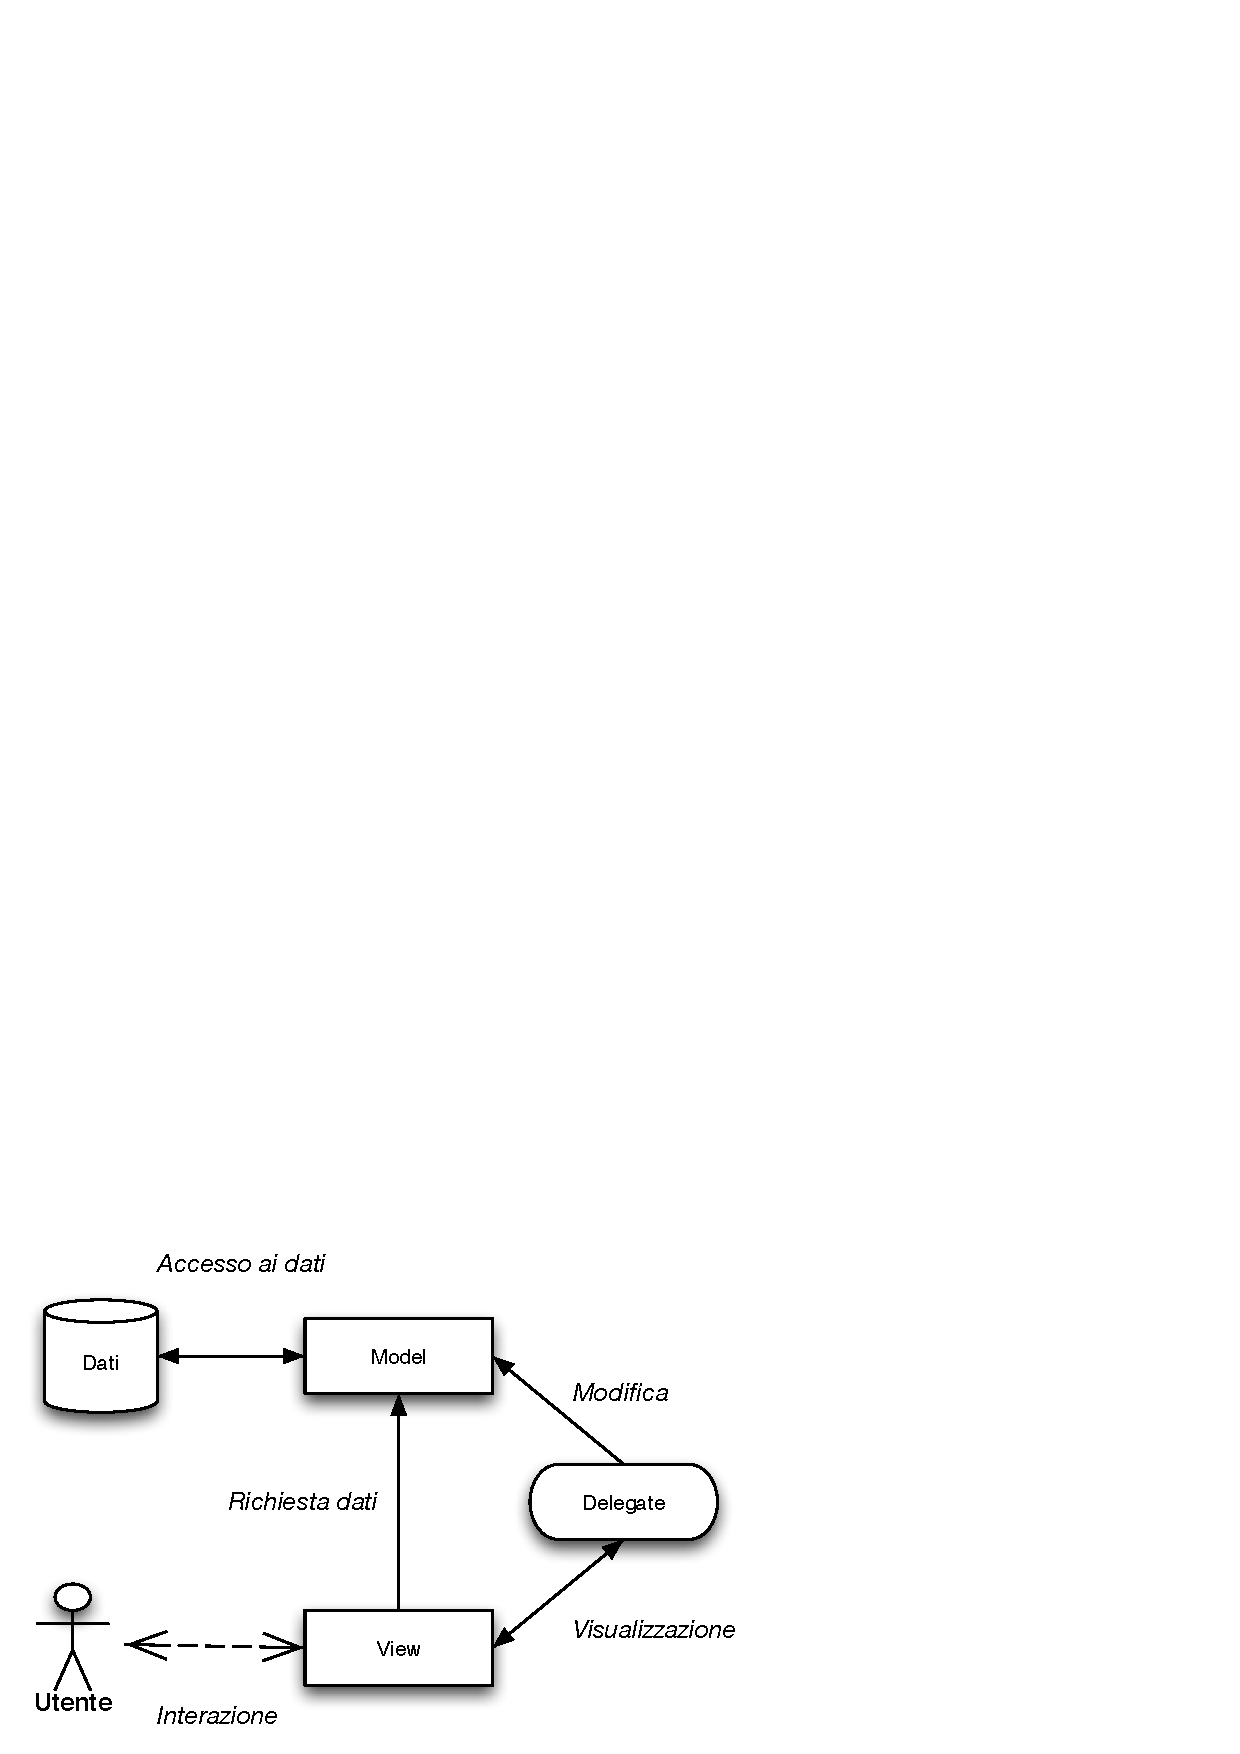
\includegraphics{images/mvd.png}
\caption{Diagramma delle interazioni nel pattern MVD in Qt}
\label{default}
\end{center}
\end{figure}


In quanto scritto finora è possibile intravedere i benefici principali che derivano dall'utilizzo di questa architettura. 

In primo luogo, è possibile presentare all'utente i dati in maniera diversa senza per questo doverli duplicare o reimplementare i metodi di accesso. Per far ciò è sufficiente realizzare più view differenti, lasciando inalterato il model. 

Viceversa, se viene a cambiare il modo in cui i dati sono memorizzati, ad esempio passando dall'uso di un semplice file di testo all'uso di un database, non sarà necessario apportare modifiche alla view, poiché questa entità è per costruzione agnostica rispetto alla strategia di accesso ai dati.

Tale architettura libera inoltre il programmatore dal compito oneroso di dover sincronizzare manualmente i dati mostrati nell'interfaccia con i dati effettivamente memorizzati, specialmente in seguito ad un'interazione dell'utente con l'interfaccia. Siccome è la view che si occupa di richiedere i dati al model nel caso in cui venga richiesta una modifica nella visualizzazione, basterà aggiornare i dati in un solo punto e la modifica verrà propagata in maniera automatica anche a tutte le view associate. 

Sussiste anche un vantaggio in termini prestazionali: siccome le view hanno consapevolezza dei dati esatti che è necessario mostrare, si limitano a richiedere quelli strettamente indispensabili in base alla visuale che l'utente ha sull'interfaccia in un determinato istante. Per fare un esempio, a fronte di qualche migliaia di record presenti nella base dati, è improbabile doverli mostrare tutti contemporaneamente all'utente in un'ipotetica tabella. Sarà la view che richiederà al model solamente il sottoinsieme di record da mostrare effettivamente quando l'utente provocherà l'evento corrispondente allo scorrimento verticale della tabella. Come risultato si ottiene una gestione più efficiente della memoria da parte dell'applicazione e un'interfaccia più reattiva.

%TODO: descrivere la possiiblità di creare in PyQt custom model e view. o di utilizzare le più comuni già presenti (treeview, etc)

\section{Il componente QtWebKit}

Come è stato detto in precedenza, si è scelto di utilizzare il framework Qt per sviluppare l'applicazione soprattuto per la possibilità di utilizzare al suo interno il motore di rendering WebKit, senza dover ricorrere a librerie esterne. Il componente QtWebKit è risultato essere ben integrato nel framework ed è stato possibile utilizzarne le potenzialità in maniera elegante ed efficace.

Siccome al centro delle funzionalità dello strumento da sviluppare si trova l'interazione con un'applicazione web, questo componente del framework ha costituito la parte principale attorno a cui gli altri moduli si trovano a ruotare.

\subsection{WebKit rendering engine}

WebKit è un motore di rendering per visualizzare documenti che utilizzando i linguaggi di markup HTML ed SVG per definire il contenuto, CSS per regolarne gli stili di visualizzazione e Javascript come linguaggio di scripting per manipolare il Document Object Model (DOM). I due componenti principali al suo interno, realizzati in C++, sono il WebCore, responsabile per il rendering dei documenti sullo schermo, e il JavaScriptCore, che implementa all'interno di WebKit l'interprete Javascript. Nelle sue ultime versioni, l'interprete Javascript in WebKit compila questo linguaggio di scripting direttamente in codice macchina, migliorando notevolmente i tempi di esecuzione.

Dopo che nel giugno 2005 Apple ha annunciato il rilascio di WebKit alla comunità open source con licenza LGPL e BSD, ne è stato effettuato il porting in svariati framework, tra qui Qt, sfruttando il fatto che WebKit, rispetto alle soluzioni alternative, si configura come un progetto più snello e modulare, quindi più facilmente integrabile.

Oltre che alla possibilità di mostrare sullo schermo le pagine web di cui è necessario verificare il comportamento, il componente QtWebKit è stato fondamentale nello sviluppo dell'applicazione per definire ed eseguire materialmente i test. Di particolare interesse si è rivelata l'interazione tra la parte di applicazione desktop in Python e la pagina web in esame. 

Grazie a questo motore di rendering è infatti stato possibile iniettare ed eseguire nel contesto della pagina web del codice Javascript generato dalla parte di applicazione in Python sotto forma di stringhe di testo, accedere e manipolare il DOM del documento tramite l'API di QtWebKit, ed infine far comunicare in maniera bidirezionale le due parti attraverso un sistema di conversione automatico da oggetti definiti in Python ad oggetti utilizzabili in Javascript all'interno della pagina web.

\subsection{Interazione tra QtWebKit ed il DOM}

Attraverso le classi \verb|QWebElement| e \verb|QWebElementCollection| il framework Qt permette al programmatore di manipolare il DOM della pagina web correntemente caricata da QtWebKit. Nello specifico, \verb|QWebElement| rappresenta un singolo nodo dell'albero del documento, e mette a disposizione i metodi per modificarne gli attributi o il contenuto, per accedere ai nodi discendenti o al nodo padre visitando l'albero DOM e per appendere ad esso nuovi elementi come suoi discendenti diretti.

I nodi del DOM sono poi selezionabili specificando un selettore CSS. E' poi possibile richiamare un metodo Javascript su di un oggetto di tipo \verb|QWebElement|, sistema utile ad esempio per simulare un evento nel DOM.

\subsection{QtWebKit Bridge}

Oltre ai metodi appena descritti, esiste un altro meccanismo all'interno del framework Qt per far comunicare l'applicazione in Python con una pagina web, Questo meccanismo, definito con il nome QWebKit  Bridge, estende l'interprete Javascript di WebKit consentendogli di lavorare con oggetti di classe \verb|QObject|, definiti all'interno del framework. 

Questa classe, che costituisce il cuore delle funzionalità di Qt, oltre a realizzare il meccanismo di eventi basato su signal e slot consente di definire proprietà per le sue istanze in maniera dinamica, ossia durante l'esecuzione del programma. Questa capacità di introspezione viene sfruttata per poter passare dinamicamente da un oggetto \verb|QObject| ad un oggetto Javascript e viceversa, data l'analogia che sussiste tra le proprietà dinamiche di entrambi. 

Naturalmente, il framework si occupa in maniera trasparente di convertire i tipi di dato da un ambiente all'altro: Qt gestisce ad esempio la conversione sia di tipi semplici, come dal tipo QString, definito nel framework, al tipo string in Javascript, sia di oggetti più complessi, come liste di tipo QList in array Javascript.

Particolarmente interessante è poi la possibilità di selezionare un nodo del DOM in uno script tramite l'API Javascript per poi passarlo al contesto Python, dove esso potrà essere manipolato sotto forma di oggetto di tipo \verb|QWebElement|. 

Allo stesso modo, anche il meccanismo di slot e signal funziona in maniera trasparente tra l'ambiente Python e quello Javascript, a patto che il signal venga definito nel contesto dell'applicazione. Dall'ambiente Javascript è consentito ad esempio stabilire una connessione tra signal e slot di due oggetti messi a disposizione dall'esterno, oppure associare ad un signal emesso in Python uno slot rappresentato da una funzione definita in un oggetto Javascript. L'unico vincolo a questo sistema molto potente di condivisione è rappresentato dal fatto che, per motivi di sicurezza, l'applicazione deve indicare in maniera esplicita quali oggetti sono accessibili al contesto Javascript.

Come si può immaginare, le interazioni appena descritte aprono numerose possibilità interessanti al programmatore, consentendogli di implementare le funzionalità progettate nel contesto a cui più si addicono. Come evidenziato nella documentazione di Qt, il confine tra l'applicazione web e quella desktop diventa molto labile e ciò permette in molti casi di sfruttare le peculiarità migliori di questi due mondi. Si possono ad esempio realizzare applicazioni web che sono mantenute per comodità su di un server remoto ed estenderne le funzionalità attraverso un'applicazione desktop che utilizza il componente QWebKit per superare le limitazioni tradizionalmente imposte da un browser, sia dal punto di vista prestazionale, sia da quello dell'interazione con il sistema operativo.

Nel nostro caso, questo interessante sistema è stato sfruttato per realizzare lo strumento di testing progettato. Uno dei vantaggi apportati, sicuramente da sottolineare, è stato riscontrato nel poter impiegare le migliori tecnologie disponibili in entrambi i contesti: per manipolare il DOM e per gestire gli eventi nell'ambiente web si è scelto di utilizzare la libreria jQuery, che offre un'interfaccia estremamente potente e concisa per questi scopi, senza doverne riscrivere da zero le funzionalità  necessarie all'interno dell'applicazione. jQuery consente di gestire il DOM e gli eventi in modo molto più efficace rispetto al componente QWebKit, perciò si è scelto di iniettare questa la logica sotto forma di codice Javascript nelle pagine web sotto esame, senza doversi preoccupare dell'interazione con la parte di codice in Python. Uno dei risultati più soddisfacenti durante lo sviluppo dello strumento per il testing è stato proprio l'alto livello di integrazione tra le tecnologie migliori a disposizione per ciascuna funzionalità da implementare.

%TODO: inserire codice?

\section{jQuery}

jQuery è una libreria in Javascript per facilitare ed uniformare tra i diversi browser la manipolazione del DOM, la gestione degli eventi, le animazioni e l'uso di richieste asincrone (AJAX). Rilasciata con doppia licenza MIT e GPL nel 2006, risulta essere ad oggi la libreria Javascript più utilizzata nel web secondo \cite{builtwith}. 

Il suo uso così diffuso è dovuto, oltre che alle prestazioni in linea con altre librerie analoghe, soprattutto all'interfaccia API semplice ed intuitiva, che permette di concentrarsi sulle funzionalità da sviluppare piuttosto che sui dettagli di basso livello. Sotto questo aspetto, jQuery si avvantaggia grazie all'implementazione di un'API di tipo \emph{fluent}, in cui è possibile concatenare di seguito più chiamate ai metodi di un oggetto, grazie al fatto che i metodi, dopo aver eseguito la manipolazione sull'oggetto, restituiscono ancora un'istanza della classe di partenza. Per rendere l'idea della leggibilità del codice scritto in jQuery, nel listato ~\ref{code:jqueryEx} viene riportato un esempio di alcune operazioni comuni.

\lstinputlisting[float=h, caption={Esempio di utilizzo della libreria jQuery}, label=code:jqueryEx ]{code/jquery_ex_1.js}

Attraverso queste poche istruzioni vengono prima selezionati i nodi del DOM di tipo DIV con classe "test", poi si accede ai rispettivi nodi figli di tipo A, che non siano però i primi nell'ordine. Di questi viene infine modificato l'attributo href ed assegnata una funzione di callback per l'evento click. 

Uno dei moduli più interessanti della libreria jQuery è proprio il sistema di selezione e di manipolazione del DOM. Nell'ambito dell'applicazione sviluppata, si è scelto di utilizzare proprio queste funzionalità di alto livello messe a disposizione dalla libreria poiché non si è riscontrato lo stesso livello di flessibilità in altre librerie sviluppate in Python.

Come visto nel capitolo relativo agli obiettivi dello strumento, due delle caratteristiche fondamentali che si è deciso di ottenere consistono nella semplicità di utilizzo e in un certo grado di robustezza dei test definiti. La scelta del sistema di selezione dei nodi del DOM nel contesto della pagina sotto esame gioca un ruolo fondamentale per il raggiungimento di entrambi questi requisiti. 

Molte delle soluzioni esistenti che sono state analizzate in fase preliminare utilizzano principalmente selettori XPath, che presentano però alcuni svantaggi rispetto ai selettori CSS. Si è deciso quindi di utilizzare i selettori CSS e si sono analizzate varie librerie che consentissero di accedere ai nodi del DOM mediante selettori CSS, valutando però anche la differente capacità espressiva rispetto all'XPath.

Inizialmente si è provato ad utilizzare la libreria PyQuery \footnote{\url{http://pypi.python.org/pypi/pyquery}}, scritta in Python, che sulla carta sembrava fornire un buon sistema di manipolazione del DOM, ispirandosi fortemente all'API di jQuery. Dopo alcuni esperimenti di utilizzo più approfondito ci si è però scontrati con alcuni bug e caratteristiche mancanti, necessarie per supportare l'algoritmo di generazione automatica dei selettori per i test sull'interfaccia della pagina web. 

Piuttosto che procedere con la correzione dei bug e l'implementazione delle caratteristiche mancanti, è sembrato più produttivo utilizzare direttamente la libreria jQuery per accedere al DOM della pagina web oggetto dei test e per implementare l'algoritmo di generazione dei selettori, sfruttando poi tecnologia QWebKit Bridge per comunicare in maniera trasparente con la parte applicativa scritta in Python.

\subsection{Un confronto tra i selettori CSS ed XPath}

Come è stato scritto in precedenza, uno dei vincoli progettuali stabiliti durante la fase di analisi dello strumento da sviluppare è stato l'utilizzo di selettori CSS piuttosto che selettori XPath per identificare gli elementi del DOM sui quali simulare gli eventi e stabilire delle assertion. Verrà presentato ora un confronto tra queste due tipologie di selettori, cercando di evidenziare gli aspetti che hanno influenzato la scelta compiuta. Per le osservazioni principali ci si è basati sugli spunti offerti in occasione della conferenza "Selenium meetup", tenutasi l'11 Maggio 2011 presso i Mozilla Office in California (\cite{suarezCss}), durante la quale si è tenuto un intervento su questo tema.

Prima di confrontare alcune caratteristiche di questi due meccanismi di selezione, è opportuno chiarire la loro differente natura per comprenderne meglio le limitazioni ed i vantaggi intrinseci.

XPath, abbreviazione di XML Path Language, è un linguaggio per la selezione dei nodi all'interno di un documento XML. La versione 1.0, standardizzata dal W3C nel 1999, nacque appunto con l'obiettivo ben specifico di fornire una sintassi per individuare un elemento nell'albero XML attraverso l'uso di un percorso simile a quello utilizzato nel formato degli URL o di un filesystem, nei quali il carattere \\ è utilizzato per separare i livelli gerarchici. 

Attraverso XPath è possibile selezionare i nodi sia rispetto ad un percorso assoluto nell'albero, sia ad uno relativo ad un altro elemento specificato. XPath è in grado inoltre di specificare percorsi sia in senso ascendente che discendente nella gerarchia rappresentata dalla struttura al albero. Il linguaggio XPath è inoltre arricchito da un corposo insieme di funzioni, che operano su stringhe, numeri e valori booleani. Esse forniscono maggiore capacità espressiva, ad esempio permettendo di selezionare elementi in base al loro contenuto, al formato della stringa contenuta in un determinato attributo, oppure di filtrare i risultati ottenuti combinando predicati di tipo logico su insiemi di nodi selezionati.

Il linguaggio CSS (Cascading Style Sheets) è invece nato per tutt'altre finalità. Esso è infatti è costituito da una serie di regole per definire l'aspetto grafico e la formattazione di un documento scritto utilizzando l'XML o i suoi formati derivati, principalmente l'HTML. Il primo standard, sviluppato dal W3C, è stato rilasciato nel 1996. Per applicare le regole di stile definite ad un certo insieme di nodi del documento, la specifica CSS definisce un sistema di selezione, che con il passare degli anni si è arricchito notevolmente di nuove caratteristiche fino all'attuale versione 3, rimanendo comunque più semplice rispetto ad XPath. 

La semplicità dei selettori CSS implica però una minore potenza rispetto ai selettori XPath (\cite{resigXpathCss}). Tra le limitazioni principali, non è possibile risalire nell'albero utilizzando un selettore CSS, ma solo specificare regole di selezione in maniera discendente, ossia da un nodo padre verso i nodi figli. Questa limitazione deriva soprattutto dal fatto che l'obiettivo principale della specifica CSS non è la selezione dei nodi e si è preferito limitarne le funzionalità a quelle di uso più comune per la presentazione dei documenti e per agevolarne un'implementazione il più omogenea possibile da parte dei vari browser. La specifica CSS definisce poi un insieme di pseudo-elementi utilizzabili nei selettori, i quali implementano però solamente un sottoinsieme delle funzionalità esprimibili tramite le funzioni di XPath.

Sebbene quindi i selettori CSS siano effettivamente meno potenti rispetto al tipo XPath, alcuni fattori ne hanno determinato la maggiore diffusione di utilizzo che è riscontrabile oggi, specialmente nell'ambito legato alle applicazioni web, come dimostrato in \cite{byeXml}.
Tra questi fattori va incluso sicuramente il progressivo abbandono del formato XML in favore di quello JSON che si è verificato negli ultimi anni. Quest'ultimo formato di codifica, essendo di fatto più maneggevole e meno verboso rispetto all'XML, ha trovato infatti largo impiego in ambito web e molti linguaggi dinamici, come Python, PHP o Ruby integrano librerie standard che forniscono un maggiore supporto all'uso questo formato. Essendo più semplice da elaborare rispetto all'XML, il formato JSON richiede una minore efficienza si adatta meglio ai linguaggi dinamici. 

\begin{figure}[htbp]
\begin{center}
\includegraphics[width=\textwidth]{images/byexml.png}
\caption{Statistica sul declino dell'uso di API in XML, tratto da \cite{byeXml}}
\label{default}
\end{center}
\end{figure}

Per citare alcuni dati pratici, sia Facebook che Twitter, nelle utlime versioni della loro API pubblica, hanno scelto di deprecare l'utilizzo dell'XML come sistema per convogliare le risposte alle richieste dei client e attualmente supportano esclusivamente il formato JSON \footnote{\url{https://dev.twitter.com/blog/changing-trends-api}} \footnote{\url{http://developers.facebook.com/docs/reference/api}}.

Ciò ha certamente portato ad un minore interesse da parte degli sviluppatori verso il linguaggio XPath, nato per essere usato in accoppiata con il formato XML. Oltretutto, i selettori CSS, benché meno potenti, sono sufficienti per gestire in maniera più semplice la grande maggioranza delle situazioni di interesse pratico.  

\subsubsection{Un confronto sulla leggibilità}

Per rendersi conto della differente leggibilità tra selettori XPath e CSS, in favore di questi ultimi, è sufficiente osservare la tabella ~\ref{table:cssVsXpath}, che mette a confronto i due tipi di selettori per lo stesso scopo. 

\begin{table}[htdp]
\caption{Confronto tra i selettori CSS e XPath}
\begin{center}
\begin{tabular}{| p{6cm} | p{8cm} |}
\hline
	\textbf{Selettore CSS} & \textbf{Selettore XPath} \\
\hline
\multicolumn{2}{|l|}{Seleziona l'elemento DIV con id "foo"} \\
\hline
	\begin{spverbatim}
		div#foo
	\end{spverbatim}
	&
	\begin{spverbatim}
		div[@id="foo"]
	\end{spverbatim} \\
\hline
\multicolumn{2}{|l|}{Seleziona l'elemento DIV che ha una classe "foo"} \\
\hline
	\begin{spverbatim}
		div.foo 
	\end{spverbatim}
	& 
	\begin{spverbatim} 
		//div[contains(concat(' ',normalize-space(@class),' '),' foo')] 
	\end{spverbatim}  \\
\hline
\multicolumn{2}{|l|}{ Seleziona l'elemento P che è il primo figlio del suo elemento padre } \\\hline
	\begin{spverbatim}
		p:first-child
	\end{spverbatim}
	&
	\begin{spverbatim}
		*[1]/self::p
	\end{spverbatim} \\
\hline
\multicolumn{2}{|l|}{Seleziona gli elementi A preceduti immediatamente da un elemento P} \\\hline
	\begin{spverbatim}
		p + a 
	\end{spverbatim}	
	& 
	\begin{spverbatim}
		p/following-sibling::*[1]/self::a
	\end{spverbatim} \\
\hline
\multicolumn{2}{|l|}{Seleziona l'elemento TD contenuto nella gerarchia specificata} \\\hline
	\begin{spverbatim}
		table#foo tr.test td:nth(2)
	\end{spverbatim}
	& 
	\begin{spverbatim}
		//table[@id="foo"]//tr[@class="test"] //td[2]
	\end{spverbatim} \\
\hline
\end{tabular}
\end{center}
\label{table:cssVsXpath}
\end{table}

Come si può osservare, i selettori CSS risultano essere nella media più semplici e di più immediata comprensione. Queste caratteristiche fanno quindi sì che i test definiti tramite selettori CSS risultino maggiormente mantenibili nel lungo periodo.

\subsubsection{Utilizzo con jQuery}

Dalla versione 1.3, la libreria jQuery ha scelto di non supportare più i selettori di tipo XPath nella sua API. L'uso di selettori CSS è quindi una scelta obbligata se si decide di impiegare jQuery senza dipendere da plugin esterni.